\begin{landscape}

\begin{minipage}{7cm}
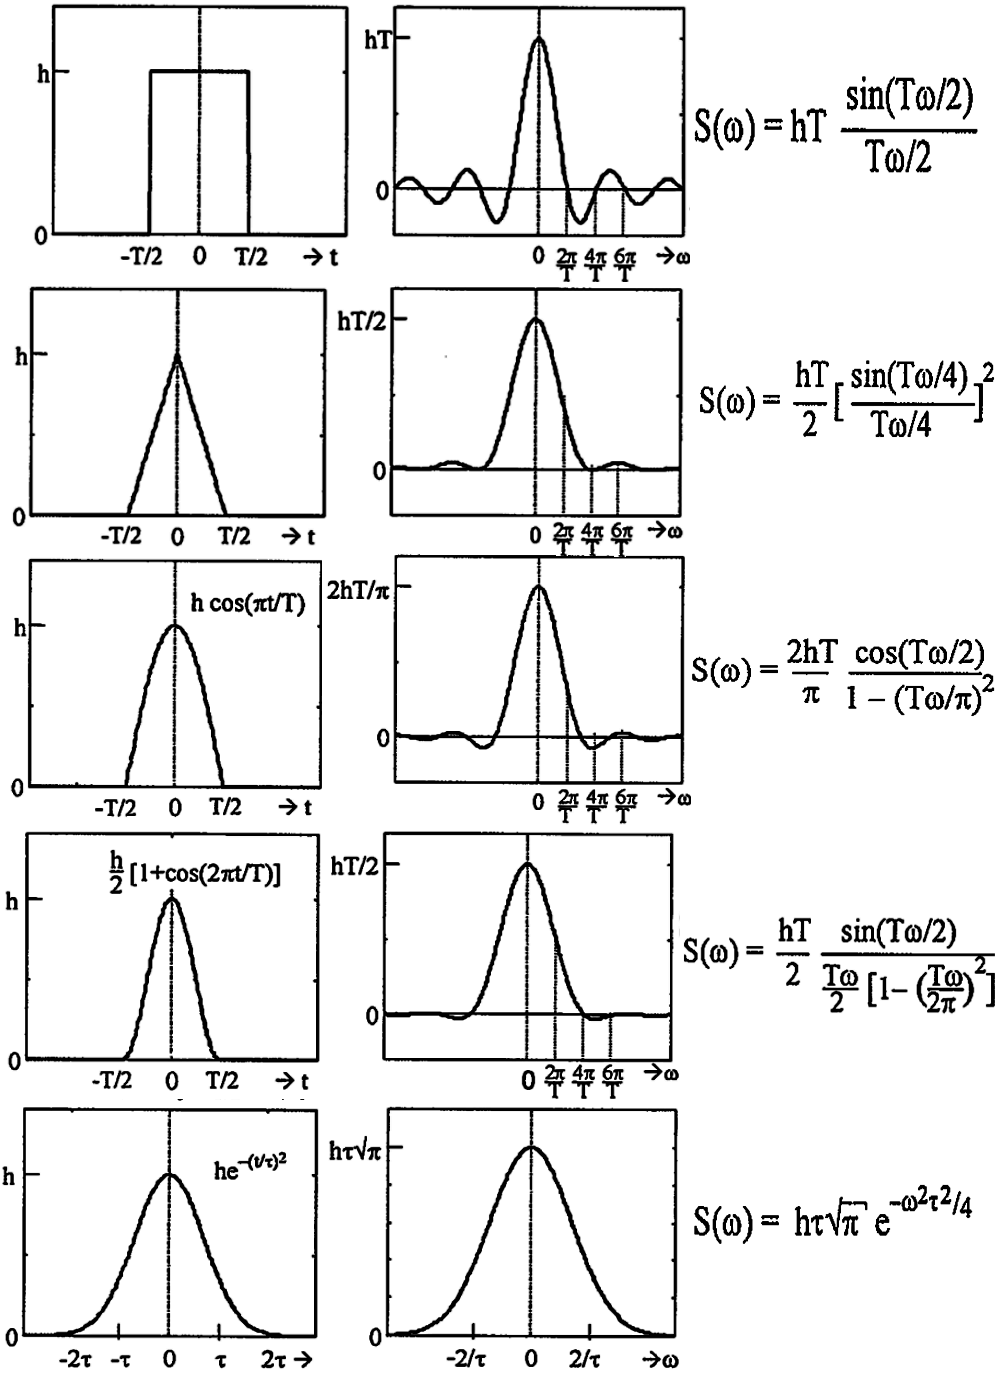
\includegraphics[width=\textwidth,trim= 0cm 0cm 0cm 0cm]{bilder/Transformationen/Fourier-Trafo.png}

\end{minipage}
\begin{minipage}{8.25cm}
	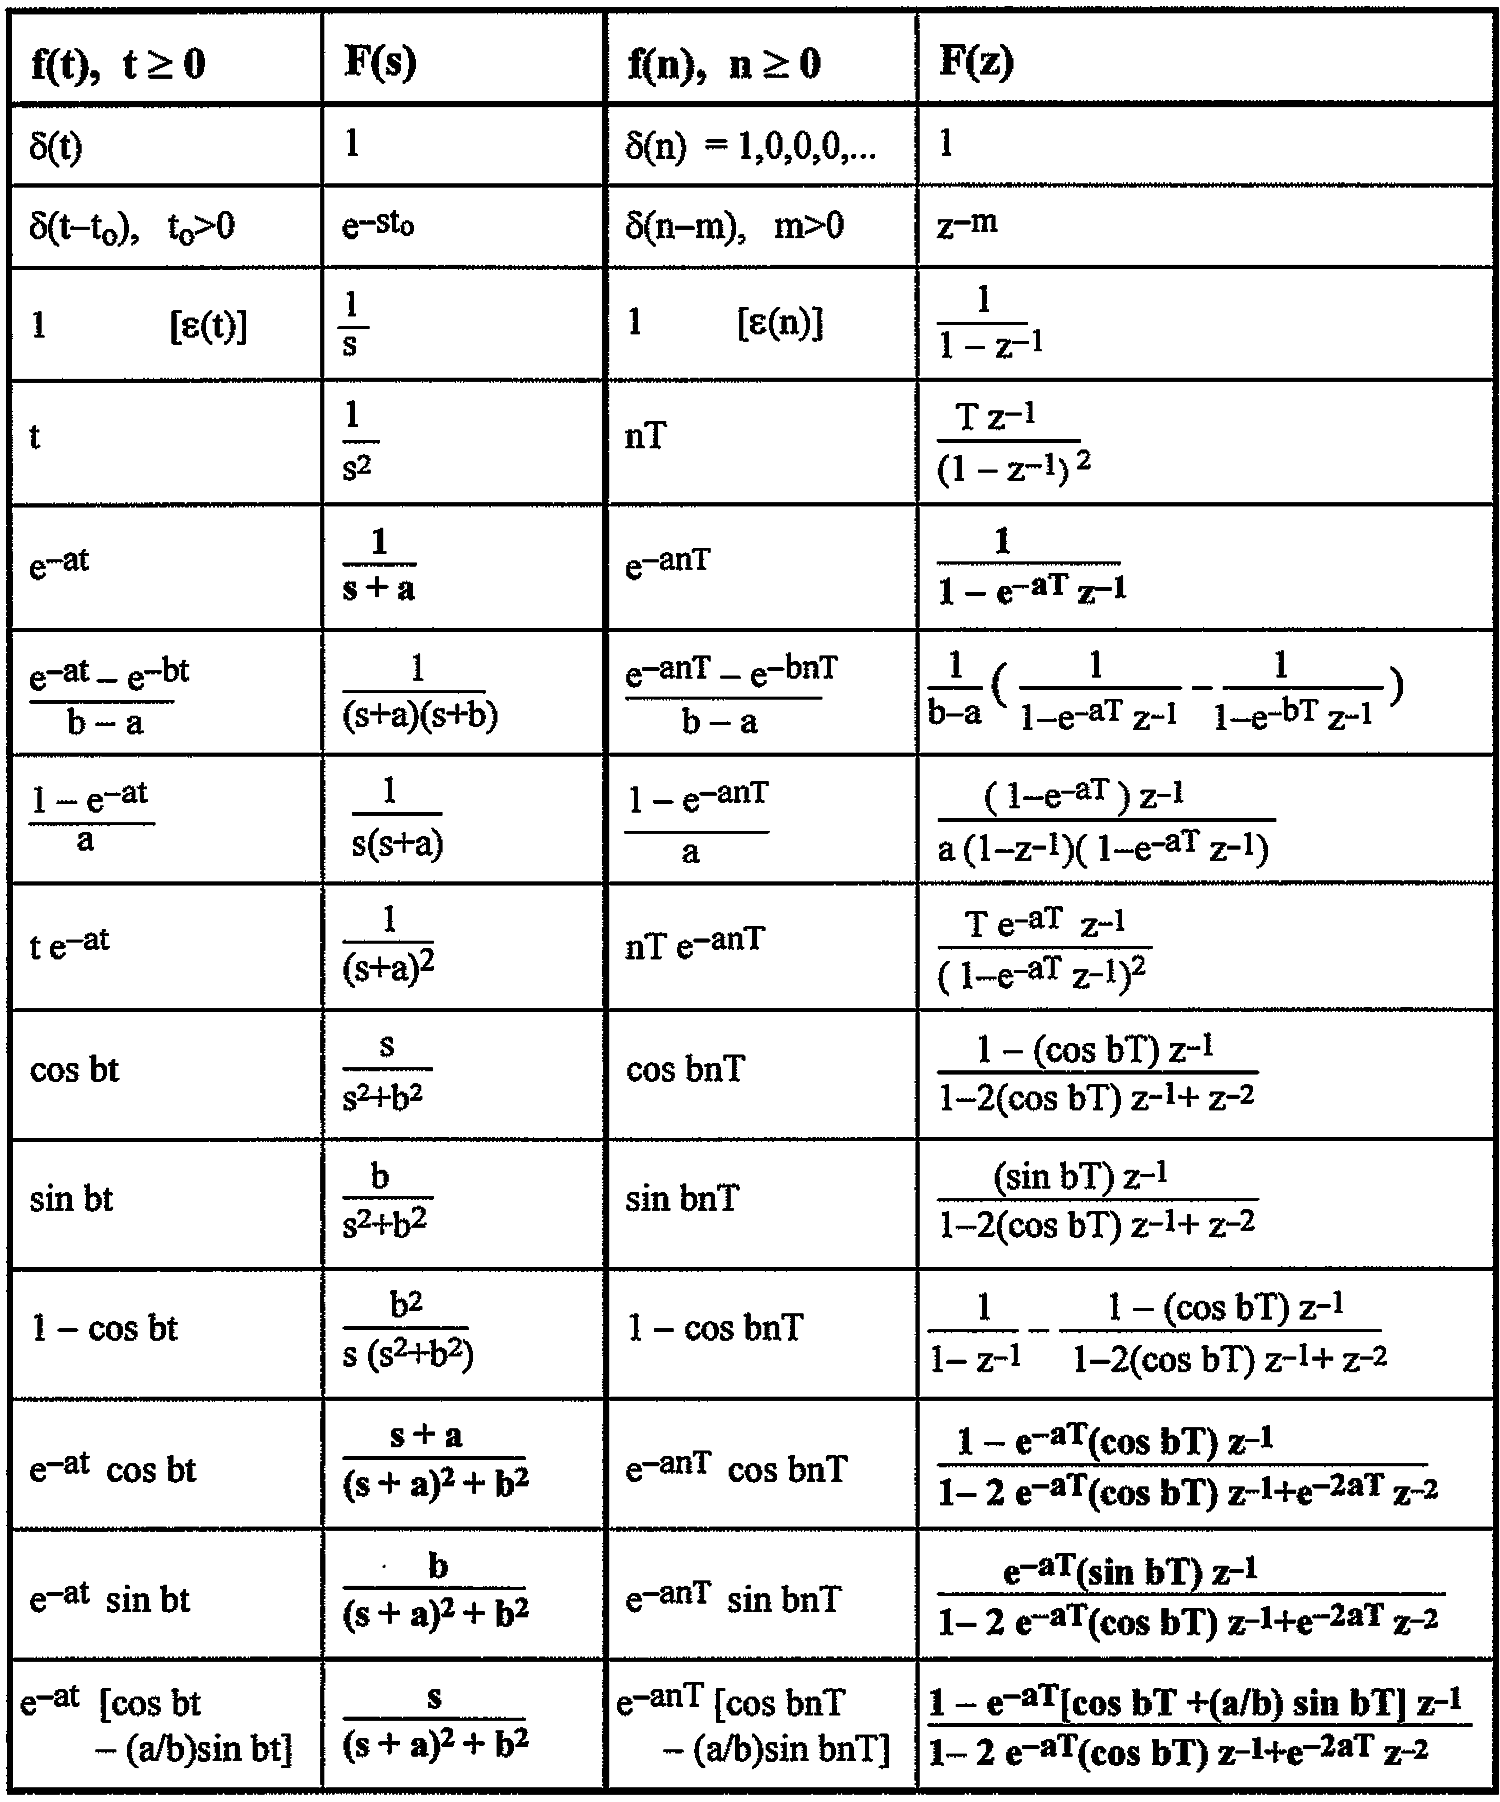
\includegraphics[width=\textwidth,trim= 0cm 0.3cm 0cm 0.45cm]{bilder/Transformationen/Z-Lexikon.png}
	\end{minipage}
	\begin{minipage}{10cm}
	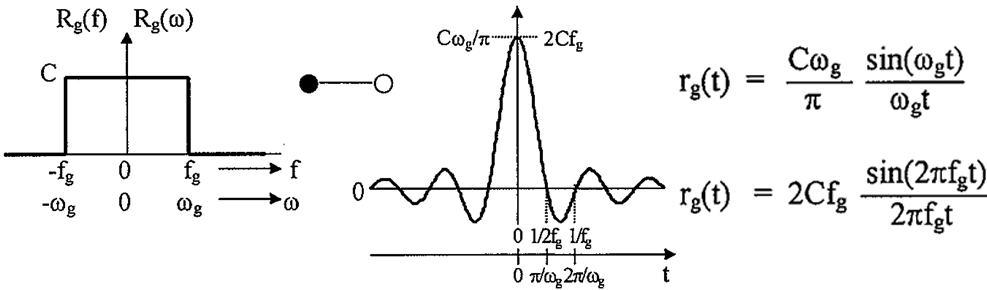
\includegraphics[width=\textwidth,trim= 0cm 0cm 0cm 0cm]{bilder/Transformationen/Rechteck-Sinc.png}
	\textbf{Matrix inversion}\\
	$A^{-1} = \begin{pmatrix}
	a & b \\ c & d \\
	\end{pmatrix}^{-1} =
	\frac{1}{\det(A)} \begin{pmatrix}
	d & -b \\ -c & a \\
	\end{pmatrix}  =
	\frac{1}{ad-bc} \begin{pmatrix}
	d & -b \\ -c & a \\
	\end{pmatrix}\quad$\\
	$A^{-1} = \begin{pmatrix}
	a & b & c\\ d & e & f \\ g & h & i \\
	\end{pmatrix}^{-1} =
	\frac{1}{\det(A)} \begin{pmatrix}
	ei - fh & ch - bi & bf - ce \\
	fg - di & ai - cg & cd - af \\
	dh - eg & bg - ah & ae - bd
	\end{pmatrix}$\\
	\begin{minipage}{4cm}
		\textbf{Trigonometry} \\
		$e^{j\varphi}=\cos(\varphi)+ j \cdot \sin(\varphi) $
		$e^{-j\varphi}=\cos(\varphi)- j \cdot \sin(\varphi) $
		$\cos(x) = \frac{e^{jx} + e^{-jx}}{2}$\\
		$\sin(x) = \frac{e^{jx} - e^{-jx}}{2j}$\\
		$\cos^2(x) = \frac12 + \frac{\cos(2x)}{2}$\\
		$\sin^2(x) = \frac12 - \frac{\cos(2x)}{2}$\\
		$\sin(2x)=2\sin(x)\cdot\cos(x)$\\
		$\sin^2(x)+\cos^2(x)=1$
	\end{minipage}
	\begin{minipage}{5cm}
		\textbf{Determinants} \\
		\footnotesize
		$\det \begin{pmatrix} a & b \\ c & d\\ \end{pmatrix} =
		a d - b c \quad$\\
		$\det \begin{pmatrix} 
		a & b & c \\
		d & e & f \\
		g & h & i  \end{pmatrix}
		= a e i + b f g + c g h \\
		\text{\hspace{2.5cm}} -c e g - f h a - i b d$		\normalsize
	\end{minipage}
\end{minipage}

%\section{Fourier Transformation}
\begin{minipage}{0.85\linewidth}
%\subsubsection{Eigenschaften von Fourier- und Z-Transformation}
\footnotesize 
\renewcommand{\arraystretch}{1.1}
\begin{tabular}{|p{4.3cm}||p{1.8cm}|p{1.8cm}||p{2.2cm}|p{2.4cm}||p{1.9cm}|p{2.6cm}|}
\hline
\textbf{Designation}
  & \multicolumn{2}{|c||}{\textbf{Time domain}}
  & \multicolumn{2}{|c||}{\textbf{Continuous frequency domain}}
  & \multicolumn{2}{|c|}{\textbf{Discrete frequency domain}} \\
  & \textbf{Continuous}
  & \textbf{Discrete}
  & \textbf{Fourier}
  & \textbf{Laplace}
  & \textbf{Discrete FT}
  & \textbf{Z Transform} \\
\hline
\hline
  Linearity 
  & $\alpha\cdot f(t) + \beta\cdot g(t)$
  & $\alpha\cdot f(n) + \beta\cdot g(n)$
  & $\alpha\cdot F(\omega) + \beta\cdot G(\omega)$
  & $\alpha\cdot F(s) + \beta\cdot G(s)$
  & $\alpha\cdot F(n) + \beta\cdot G(n)$
  & $\alpha\cdot F(z) + \beta\cdot G(z)$\\
\hline
  Similarity / Time scaling or reflection about the Y-axis
  &	$f(\alpha t)$ 
  & $f(-n)$
  & $\frac{1}{|\alpha|}F \left (\frac{\omega}{\alpha} \right)$
  & $\frac{1}{\alpha}F \left (\frac{s}{\alpha} \right )$ 
  & $F(-n)$
  & $F(z^{-1})$\\
%\hline
  %Damping
  %& -
  %& $e^{dn} f(n)$
  %& -
  %& - 
  %& -
  %& $F(z e^{d})$ \\
\hline
  Shift in the time domain 
  & $f(t\pm t_0)$ 
  & $f(n \pm n_0)$
  & $e^{\pm j\omega t_0} F(\omega)$
  & $F(s)e^{\pm t_0 s}$ 
  & $e^{\pm j\frac{n}{N}2 \pi n_0} F(n)$
  & $z^{\pm n_0} F(z)$\\
\hline
Shift in the frequency domain 
  & $f(t)e^{\mp\alpha t}$ 
  & $f(n) e^{\mp j \frac{n}{N} 2 \pi n_0}$
  & $F(\omega\pm \alpha)$
  & $F(s\pm\alpha)$ 
  & $F(n \pm n_0)$
  & $F(z \pm n_0)$\\
\hline
Convolution in the time domain 
  &	$f(t) \ast g(t)$
  & $f(n) \ast g(n)$
  & $F(\omega) \cdot G(\omega)$
  & $F(s) \cdot G(s)$
  & $F(n) \cdot G(n)$ 
  & $F(z) \cdot G(z)$ \\
\hline
  Convolution in the frequency domain 
  &	$f(t) \cdot g(t)$
  & $f(n) \cdot g(n)$
  & $\frac{1}{2\pi} F(\omega) \ast G(\omega)$
  & $\frac{1}{2\pi} F(s) \ast G(s)$ 
  & $\frac{1}{N} F(n) \ast G(n)$
  & $\frac{1}{N} F(z) \ast G(z)$\\
\hline
  Derivatives in the time domain / difference formation 
  & $\frac{\partial^n f(t)}{\partial t^n}$ 
  & $\Delta^k f(n)$
  & $(j\omega)^n F(\omega)$
  & $s^nF(s)-s^{n-1}f(0+)-s^{n-2}\frac{\partial f(0+)}{\partial t}-\ldots
 			-s^0\frac{\partial^{n-1} f(0+)}{\partial t^{n-1}}$
  & 
  & $(1-z^{-1})^k F(z)$ \\
\hline
  Derivative in the frequency domain
  & $(-t)^k\cdot f(t)$ 
  & $n f(n)$ 
  & $j^k \frac{-\partial^k F(\omega)}{\partial \omega^k}$
  & $\frac{\partial^k F(s)}{\partial s^k}$
  & 
  & $-z \frac{\partial F(z)}{\partial z}$ \\
\hline 			
  Integration / Summation
  & $\int\limits_{-\infty}^t f(\tau)d\tau$ 
  & $\sum\limits_{n=0}^{k} f(n)$
  & $\frac{F(\omega)}{j\omega}+F(0)\pi\delta(\omega)$
  & $\frac{F(s)}{s}$
  & 
  & $\frac{1}{1-z^{-1}} F(z)$ \\
\hline
  Initial value 
  & $\lim\limits_{t\rightarrow 0} f(t)$ 
  & $f(0)$
  & 
  & $\lim\limits_{s\rightarrow \infty} sF(s)$ 
  & 
  & $\lim\limits_{z \rightarrow \infty} F(z)$ \\
\hline
  Final value
  &	$\lim\limits_{t\rightarrow \infty} f(t)$
  & $\lim\limits_{n\rightarrow \infty} f(n)$
  & 
  & $\lim\limits_{s\rightarrow 0} sF(s)$
  & 
  & $\lim\limits_{z \rightarrow 1} (1-z^{-1}) F(z))$\\
%\hline
  %Stability
  %& -
  %& -
  %& -
  %& Pole in LHP
  %& 
  %& Pole inside unit circle \\
%\hline
  %Causality
  %& -
  %& -
  %& A- \& Causal
  %& Only Causal
  %& 
  %& $\lim\limits_{z \rightarrow \infty} z^{-1} F(z) = 0$ \\
\hline
\hline
  Special
  & \multicolumn{3}{l||}{
      Bessel's theorem \qquad
      $\int\limits_{-\infty}^{\infty}f(t)g^{\ast}(t)dt =
         \frac{1}{2\pi}
         \int\limits_{-\infty}^{\infty}F(\omega)G^{\ast}(\omega)d\omega$}
  & \multicolumn{3}{|l|}{
      Parseval's theorem \qquad
      $W = \int\limits_{-\infty}^{\infty}|f(t)|^2 dt = \frac{1}{2\pi}
      \int\limits_{-\infty}^{\infty}|F(\omega)|^2 d\omega$
    }\\
\hline
\end{tabular}
\end{minipage}
\begin{minipage}{0.2\linewidth}
\textbf{Quadratic Equation:}\\
$a\cdot x^2+b\cdot x +c=0$\\

$x_{1,2}=\frac{-b\pm \sqrt{b^2-4ac}}{2a}$\\

\textbf{Fourier Transform:}\\

$\delta(t)\FT 1$\\
$1\FT 2\pi \delta(\omega)$\\
$\sigma(t)\FT \frac{1}{j\omega}+\pi\delta(\omega)$\\
$\text{sgn}(t)\FT \frac{2}{j\omega}$\\
$e^{\pm j \omega_0 t} \FT 2\pi \delta(\omega \mp \omega_0)$\\
$\sin(\omega_0t)\FT j\pi(\delta(\omega +\omega_0)-\newline\text{\hspace{2.7cm}}\delta(\omega -\omega_0))$\\
$\cos(\omega_0t)\FT \pi(\delta(\omega +\omega_0)+\newline\text{\hspace{2.6cm}}\delta(\omega -\omega_0))$\\
\end{minipage}


%% We don't need this and it does not fit onto the page. The trigonometric relationships are already on this page under ''Trigonometrie'', and the z-transforms are in the z-transform table. 
%% In my opinion the z-transform table should also be updated, because you can barely read it when it's included as a picture and scaled. 
 
% \begin{minipage}{\linewidth}
% \vspace*{-1cm}
% $e^{j\omega}=\cos(\omega) + j \cdot \sin(\omega)$
% \quad
% $\sin(\omega)=\dfrac{e^{j\omega} - e^{-j\omega}}{2j}$
% \quad
% $\cos(\omega)=\dfrac{e^{j\omega} + e^{-j\omega}}{2}$
% \quad
% $1\pm e^{-j\omega T}= (e^{j\frac{\omega}{2} T}\pm e^{-j\frac{\omega}{2} T})\cdot e^{-j\frac{\omega}{2} T}$
% \quad
% $a^n \FT \frac{1}{1-az^-1}$
% \quad
% $a^{|n|} \FT \frac{1-a^2}{(1-az^-1)(1-az)}$
% \quad
% \vspace*{-2cm}
% \end{minipage}


\end{landscape}